\documentclass[12pt]{article}

\usepackage[utf8]{inputenc}
\usepackage[T1]{fontenc}
\usepackage{amsmath, amssymb, amsthm}
\usepackage{geometry}
\usepackage[unicode]{hyperref}
\usepackage{booktabs}
\usepackage{enumitem}
\usepackage{tikz}
\usetikzlibrary{automata, positioning, arrows.meta, calc}

\geometry{margin=1in}

\setlength{\parindent}{0pt}
\setlength{\parskip}{1em}

\newtheorem{definition}{Definition}
\newtheorem{remark}{Remark}

\title{Waterworks Asset Rehabilitation as a Restless Bandit Problem:\\Risk-Constrained Cost Minimization}
\author{Gregory Zancewicz}
\date{February 2026}

\begin{document}

\maketitle

\begin{abstract}
This document provides a formal mathematical specification for a waterworks asset rehabilitation problem modeled as a restless bandit with an aggregate risk constraint. The system consists of $N_a$ infrastructure assets across $N_c$ classes, each subject to stochastic failure governed by a class-specific Weibull distribution parameterized by shape $\beta_j$ and scale $\eta_j$. Each asset has two operational states---Operating and Failed---with a continuously tracked effective age driving the failure hazard. A Likelihood of Failure (LoF) score derived from the Weibull cumulative failure probability and a fixed Consequence of Failure (CoF) score are combined into an Asset Risk score, stratified into five Risk Levels. The planner's objective is to \emph{maximize reward} (equivalently, minimize intervention cost) subject to maintaining the system's aggregate Risk Level at or below a target threshold. The optimal policy's cost then determines the required maintenance budget. We define the state space, transition kernel, risk scoring, objective function, and constraint structure, then describe in detail how the Whittle index policy provides a tractable, near-optimal solution approach.
\end{abstract}

\tableofcontents
\newpage

%% ============================================================
\section{Problem Description}
%% ============================================================

This paper presumes some familiarity with Markov decision processes (MDPs) and multi-armed bandit processes. For background on these topics, including formal definitions and worked examples, the reader is referred to Zancewicz~\cite{zancewicz2026mdp}.

A water utility manages $N_a$ infrastructure assets (pipes, valves, pump stations, treatment components, etc.) drawn from $N_c$ asset classes. Each class $j \in \{1, \dots, N_c\}$ shares common physical characteristics: a Weibull shape parameter $\beta_j > 1$ and scale parameter $\eta_j$ governing the failure hazard, a rehabilitation cost $c_j$, and a replacement cost $C_j > c_j$. Each individual asset $k$ additionally carries a fixed \textbf{Consequence of Failure} score $\text{CoF}_k \in \{1, \dots, 10\}$, reflecting the community impact of its failure (proximity to schools, hospitals, major roads, population density, etc.). This score is not a monetary quantity.

Assets are subject to stochastic failure whether or not they receive maintenance: the failure hazard increases with age according to the Weibull distribution. At each decision epoch (one week), the planner may rehabilitate or replace at most $L$ assets total, drawn from a shared labor pool. Rehabilitation resets an operating asset to ``good as new'' condition (effective age zero) at cost $c_j$; replacement of a failed asset achieves the same reset at the higher cost $C_j$. Failed assets remain out of service until actively replaced.

The planner's objective is to \textbf{maximize reward} (minimize total intervention cost) subject to maintaining an aggregate measure of system risk at or below a prescribed threshold. The optimal policy reveals the minimum cost---and therefore the required annual maintenance budget---needed to achieve a given risk target.

Note that this formulation does not currently incorporate inspections or condition assessments as decision actions; all state information is assumed to be available to the planner at each epoch. Incorporating inspection scheduling as an additional action is left for future work.

The planner's objective in this paper is to minimize cost subject to an aggregate (mean) Risk Level constraint, as described in Section~\ref{sec:objective}. In future work, we intend to adapt the model to enforce a \emph{maximum acceptable Risk Level} per asset, which would provide stricter per-asset guarantees at the expense of higher required budgets.

This problem is a \textbf{restless bandit}: every asset's condition evolves at every time step regardless of whether it is acted upon, and a capacity constraint limits the number of simultaneous interventions.

%% ============================================================
\section{State Space and Risk Scoring}
\label{sec:state}
%% ============================================================

\subsection{Per-Asset State}

Each asset $k$ has an \textbf{operational state} and an \textbf{effective age}:
\begin{itemize}
  \item \textbf{Operational state} $o_k \in \{\texttt{O}, \texttt{F}\}$: the asset is either \texttt{O}perating or \texttt{F}ailed.
  \item \textbf{Effective age} $\tau_k \geq 0$: the time (in years) elapsed since the asset was last rehabilitated, replaced, or installed. This is a continuous quantity that increases deterministically by $\Delta = 1/52$ years each week.
\end{itemize}

The full per-asset state is the pair $(o_k, \tau_k)$. An operating asset ages and faces increasing failure risk; a failed asset is frozen at $o_k = \texttt{F}$ until replaced.

Figure~\ref{fig:markov-chain} shows the Markov chain structure of a single asset. The two operational states are connected by stochastic failure (Operating $\to$ Failed, with age-dependent probability $p_{\text{fail}}(\tau)$) and deterministic self-loops (an operating asset that survives remains operating with incremented age; a failed asset stays failed).

\begin{figure}[ht]
\centering
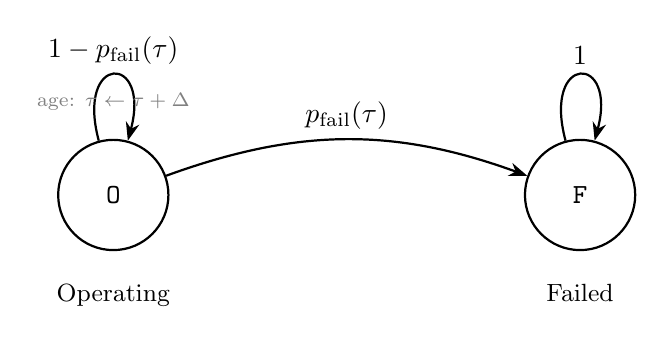
\begin{tikzpicture}[
    ->,
    >=Stealth,
    node distance=4.5cm,
    every state/.style={thick, minimum size=1.4cm},
    every edge/.style={draw, thick},
  ]
  % States
  \node[state] (O) {$\texttt{O}$};
  \node[state] (F) [right=of O] {$\texttt{F}$};

  % Labels below states
  \node[below=3mm] at (O.south) {\small Operating};
  \node[below=3mm] at (F.south) {\small Failed};

  % Transitions
  \path (O) edge [loop above, looseness=8]
            node[above] {$1 - p_{\text{fail}}(\tau)$}
            node[below=1mm, anchor=north, font=\scriptsize, text=gray] {age: $\tau \leftarrow \tau + \Delta$} (O);
  \path (O) edge [bend left=20]
            node[above] {$p_{\text{fail}}(\tau)$} (F);
  \path (F) edge [loop above, looseness=8]
            node[above] {$1$} (F);
\end{tikzpicture}
\caption{Markov chain for a single asset under the passive action ($a = 0$). The failure probability $p_{\text{fail}}(\tau)$ increases with effective age $\tau$ according to the Weibull hazard. A failed asset remains failed (absorbing state) until actively replaced.}
\label{fig:markov-chain}
\end{figure}

\subsection{Discretization of Effective Age}
\label{sec:discretization}

For computational purposes, the continuous effective age $\tau_k$ is discretized into $n$ bins. Let $\tau_{\max,j}$ be a chosen upper bound on the effective age for class $j$ (e.g., $2 \cdot \eta_j$ or a value beyond which survival probability is negligible). The age bins are:
\begin{equation}
  \mathcal{B}_j = \left\{\left[\frac{(i-1)\,\tau_{\max,j}}{n},\; \frac{i\,\tau_{\max,j}}{n}\right) : i = 1, \dots, n\right\},
\end{equation}
with representative ages $\bar{\tau}_i = (i - \tfrac{1}{2})\,\tau_{\max,j}/n$ for each bin $i$. The number of bins $n$ is a resolution parameter chosen by the modeler; larger $n$ gives a finer approximation at the cost of a larger single-arm MDP.

Including the failed state, the discrete state space for each arm is
\begin{equation}
  \mathcal{S} = \{1, 2, \dots, n\} \cup \{\texttt{F}\},
\end{equation}
with $|\mathcal{S}| = n + 1$. State $i \in \{1, \dots, n\}$ means the asset is operating with effective age in bin $i$; state $\texttt{F}$ means the asset has failed.

\subsection{Weibull Failure Model}
\label{sec:weibull}

Each asset class $j$ has time-to-failure distributed as $\text{Weibull}(\beta_j, \eta_j)$ with shape $\beta_j > 1$ (modeling wear-out) and scale $\eta_j > 0$. The cumulative failure probability by effective age $\tau$ is
\begin{equation}
  F_j(\tau) = 1 - \exp\!\left[-\left(\frac{\tau}{\eta_j}\right)^{\beta_j}\right],
\end{equation}
the survival function is $S_j(\tau) = 1 - F_j(\tau)$, and the hazard rate (instantaneous failure rate conditional on survival to age $\tau$) is
\begin{equation}
  h_j(\tau) = \frac{\beta_j}{\eta_j}\left(\frac{\tau}{\eta_j}\right)^{\beta_j - 1}.
\end{equation}
Since $\beta_j > 1$, the hazard is increasing: older assets fail at a higher rate, consistent with wear-out degradation.

\begin{remark}
If the Weibull parameters are specified via a median life $L_{50,j}$ and shape $\beta_j$, the scale parameter is determined by
\begin{equation}
  \eta_j = \frac{L_{50,j}}{(\ln 2)^{1/\beta_j}},
\end{equation}
since $F_j(L_{50,j}) = 0.5$ by definition of the median life.
\end{remark}

\subsection{Likelihood of Failure Score}

The \textbf{Likelihood of Failure} (LoF) score for asset $k$ of class $j$ is derived from the Weibull cumulative failure probability evaluated at the asset's effective age:
\begin{equation}
  \text{LoF}_k = 1 + 9 \cdot F_j(\tau_k).
  \label{eq:lof}
\end{equation}
This maps a new asset ($\tau_k = 0$, $F_j = 0$) to $\text{LoF}_k = 1$ (lowest likelihood) and an asset whose cumulative failure probability approaches 1 to $\text{LoF}_k = 10$ (highest likelihood). For the discrete bins, the LoF score at bin $i$ uses the representative age: $\text{LoF}(i) = 1 + 9 \cdot F_j(\bar{\tau}_i)$. A failed asset ($o_k = \texttt{F}$) is assigned $\text{LoF}_k = 10$.

\begin{remark}
Unlike a linear damage fraction model, the LoF score inherits the Weibull CDF's nonlinear shape. For $\beta_j > 1$ the score increases slowly at first (when the hazard is low) and accelerates as the asset ages into the wear-out region. This directly reflects the actual failure likelihood rather than a linear approximation.
\end{remark}

\subsection{Asset Risk and Risk Level}

The \textbf{Asset Risk} score for asset $k$ is the sum of its likelihood and consequence scores:
\begin{equation}
  \text{AR}_k = \text{LoF}_k + \text{CoF}_k.
\end{equation}
Since $\text{LoF}_k \in [1, 10]$ and $\text{CoF}_k \in \{1, \dots, 10\}$, the Asset Risk ranges from $2$ to $20$.

The Asset Risk is stratified into five \textbf{Risk Levels}:

\begin{center}
\begin{tabular}{ccc}
  \toprule
  Risk Level & Label & Asset Risk Range \\
  \midrule
  1 & Negligible & $[2,\; 5.6)$ \\
  2 & Low & $[5.6,\; 9.2)$ \\
  3 & Moderate & $[9.2,\; 12.8)$ \\
  4 & High & $[12.8,\; 16.4)$ \\
  5 & Extreme & $[16.4,\; 20]$ \\
  \bottomrule
\end{tabular}
\end{center}

The bin boundaries are evenly spaced across the $[2, 20]$ range. Alternatively, the boundaries may be set by policy to reflect operational risk tolerance.

\begin{remark}
The Risk Level of asset $k$ depends on both its effective age (through $\text{LoF}_k$) and its fixed $\text{CoF}_k$. Two assets of the same age may have different Risk Levels if their CoF scores differ. An asset near a school ($\text{CoF} = 9$) with low cumulative failure probability ($\text{LoF} \approx 2$) has $\text{AR} \approx 11$ (Moderate), while the same asset near end of life ($\text{LoF} \approx 9$) has $\text{AR} \approx 18$ (Extreme).
\end{remark}

\subsection{Joint State}

The global state at decision epoch $t$ is the vector $\mathbf{s}^t = (s_1^t, s_2^t, \dots, s_{N_a}^t) \in \mathcal{S}^{N_a}$, where each $s_k^t$ is a discrete age bin or $\texttt{F}$. The joint state space has $(n+1)^{N_a}$ elements, which is astronomically large for any realistic $N_a$. This exponential blowup is the fundamental reason exact dynamic programming is intractable and motivates the Whittle index decomposition described in Section~\ref{sec:whittle}.

%% ============================================================
\section{MDP Formulation}
\label{sec:transitions}
%% ============================================================

\subsection{Markov Decision Process}

A \textbf{Markov Decision Process} (MDP) is a mathematical framework for sequential decision-making under uncertainty. An MDP is defined by a tuple $(\mathcal{S}, \mathcal{A}, P, R, \gamma)$:
\begin{itemize}
  \item $\mathcal{S}$: a finite set of \textbf{states}.
  \item $\mathcal{A}$: a finite set of \textbf{actions} available to the decision-maker.
  \item $P(s' \mid s, a)$: the \textbf{transition kernel}---the probability of moving to state $s'$ given current state $s$ and action $a$. This encodes the Markov property: the next state depends only on the current state and the action taken, not on the history.
  \item $R(s, a)$: the \textbf{reward} (or cost) received when taking action $a$ in state $s$.
  \item $\gamma \in [0, 1)$: the \textbf{discount factor}, which weights future rewards relative to immediate ones.
\end{itemize}
At each decision epoch, the system is in some state $s \in \mathcal{S}$. The decision-maker selects an action $a \in \mathcal{A}$, receives reward $R(s, a)$, and the system transitions to a new state $s'$ drawn from $P(\cdot \mid s, a)$. A \textbf{policy} $\pi : \mathcal{S} \to \mathcal{A}$ maps states to actions. The goal is to find a policy that maximizes the expected discounted cumulative reward $\mathbb{E}_\pi[\sum_{t=0}^{\infty} \gamma^t R(s^t, a^t)]$.

\subsection{Single-Asset MDP}

For a single asset $k$ of class $j$, the MDP components are:
\begin{itemize}
  \item \textbf{States:} $\mathcal{S} = \{1, 2, \dots, n, \texttt{F}\}$ (age bins plus failed).
  \item \textbf{Actions:} $\mathcal{A} = \{0, 1\}$ (passive or active).
  \item \textbf{Transitions:} $P(s' \mid s, a)$ defined below.
  \item \textbf{Reward:} $R(s, a)$ as defined in Section~\ref{sec:objective}.
  \item \textbf{Discount:} $\gamma = (1 + r_{\text{ann}})^{-1/52}$.
\end{itemize}

\begin{remark}[Stationarity]
In the continuous-age formulation, the failure probability $p_{\text{fail},j}(\tau)$ depends on the asset's effective age $\tau$, which changes every epoch. This means the transition probabilities are \emph{not} time-homogeneous when viewed as a function of calendar time---an asset's failure risk at epoch $t$ depends on how long it has been since its last rehabilitation.

However, once the effective age is discretized into bins, the age becomes part of the state: state $i$ encodes both the operational status (operating) and the age range. The transition probabilities $P(s' \mid i, a)$ then depend only on the current state $i$ and action $a$, not on calendar time $t$. The discretized MDP is therefore \textbf{stationary} (time-homogeneous). This is the standard technique for converting a process with time-varying dynamics into a stationary MDP: expand the state space to include the time-varying quantity as a state variable. Stationarity is required for the Whittle index theory (Section~\ref{sec:whittle}) to apply, since the index of a state must be a fixed quantity independent of the decision epoch.
\end{remark}

The decision epoch is one week ($\Delta = 1/52$ years). Figure~\ref{fig:mdp-diagram} illustrates the decision structure: from each state, the agent chooses an action, and the action--state pair determines a probability distribution over next states.

\begin{figure}[ht]
\centering
\begin{tikzpicture}[
    ->,
    >=Stealth,
    state/.style={circle, draw, thick, minimum size=1.6cm},
    sa/.style={rectangle, draw, dotted, thick, inner sep=3pt, font=\small},
    every edge/.style={draw, thick},
  ]
  %% --- State nodes (large circles) ---
  \node[state] (O) at (0, 0) {$\texttt{O}$};
  \node[state] (F) at (7, 0) {$\texttt{F}$};

  %% --- (s, a) nodes (dotted rectangles) ---
  % Above O: passive
  \node[sa] (Oa0) at (0, 2.2) {$\texttt{O},\, a{=}0$};
  \node[above=2mm, font=\scriptsize] at (Oa0.north) {$r = 0$};
  % Below O: active
  \node[sa] (Oa1) at (0, -2.2) {$\texttt{O},\, a{=}1$};
  \node[below=2mm, font=\scriptsize] at (Oa1.south) {$r = -c_j$};
  % Above F: passive
  \node[sa] (Fa0) at (7, 2.2) {$\texttt{F},\, a{=}0$};
  \node[above=2mm, font=\scriptsize] at (Fa0.north) {$r = 0$};
  % Below F: active
  \node[sa] (Fa1) at (7, -2.2) {$\texttt{F},\, a{=}1$};
  \node[below=2mm, font=\scriptsize] at (Fa1.south) {$r = -C_j$};

  %% --- Edges: states to (s,a) nodes ---
  \draw (O) -- (Oa0);
  \draw (O) -- (Oa1);
  \draw (F) -- (Fa0);
  \draw (F) -- (Fa1);

  %% --- Transition edges from (s,a) to next states ---

  % O, a=0: survive -> O, fail -> F
  \draw (Oa0) to[out=150, in=120, looseness=4]
    node[left, font=\small, pos=0.5] {$1 - p_{\text{fail}}$} (O);
  \draw (Oa0) --
    node[above, font=\small, pos=0.5] {$p_{\text{fail}}$} (F);

  % O, a=1: reset -> O (back to self, age 0)
  \draw (Oa1) to[out=210, in=240, looseness=4]
    node[left, font=\small, pos=0.5] {$1$} (O);

  % F, a=0: stay failed -> F
  \draw (Fa0) to[out=30, in=60, looseness=4]
    node[right, font=\small, pos=0.5] {$1$} (F);

  % F, a=1: replace -> O
  \draw (Fa1) --
    node[below, font=\small, pos=0.5] {$1$} (O);
\end{tikzpicture}
\caption{MDP transition diagram for a single asset. Large circles are states ($\texttt{O}$ = Operating, $\texttt{F}$ = Failed). Dotted rectangles are state--action pairs $(s, a)$ with associated rewards $r$. Arrows from $(s, a)$ nodes to states are labeled with transition probabilities. The failure probability $p_{\text{fail}} = p_{\text{fail},j}(\tau)$ depends on the asset's current effective age.}
\label{fig:mdp-diagram}
\end{figure}

\subsection{Passive Transitions ($a_k = 0$: Do Nothing)}

Under the passive action, an operating asset ages by $\Delta$ and may fail stochastically. The conditional probability of failure during one week, given survival to current age $\tau$, is
\begin{equation}
  p_{\text{fail},j}(\tau) = 1 - \frac{S_j(\tau + \Delta)}{S_j(\tau)} = 1 - \exp\!\left[-\left(\frac{\tau + \Delta}{\eta_j}\right)^{\beta_j} + \left(\frac{\tau}{\eta_j}\right)^{\beta_j}\right].
\end{equation}
This probability increases with $\tau$, reflecting the increasing Weibull hazard.

For a discrete age bin $i$ with representative age $\bar{\tau}_i$, the passive transition probabilities are:
\begin{align}
  P(\texttt{F} \mid i,\, a{=}0) &= p_{\text{fail},j}(\bar{\tau}_i), \label{eq:pfail} \\
  P(i' \mid i,\, a{=}0) &= \big(1 - p_{\text{fail},j}(\bar{\tau}_i)\big) \cdot q(i' \mid i), \quad i' \in \{1, \dots, n\},
\end{align}
where $q(i' \mid i)$ is the deterministic or near-deterministic age advance: the asset's effective age increases by $\Delta$, so it either remains in bin $i$ or advances to bin $i{+}1$ (or stays in bin $n$ if already at the upper boundary).

\begin{remark}
From state $\texttt{F}$ (Failed), the passive transition is $P(\texttt{F} \mid \texttt{F},\, a{=}0) = 1$: a failed asset remains failed until actively replaced.
\end{remark}

\subsection{Active Transitions ($a_k = 1$: Rehabilitate or Replace)}

Rehabilitation (from operating states) or replacement (from state $\texttt{F}$) resets the asset to ``good as new'' ($\tau_k \leftarrow 0$):
\begin{equation}
  P(1 \mid s,\, a{=}1) = 1 \quad \text{for all } s \in \mathcal{S}.
\end{equation}
The effective age is reset to zero (bin 1) and the Weibull clock restarts.

%% ============================================================
\section{Objective, Reward, and Constraints}
\label{sec:objective}
%% ============================================================

\subsection{Reward Structure (Negative Cost)}

The planner's reward is the negative of intervention spending. At each epoch $t$, the per-asset reward is:
\begin{equation}
  R_k(s_k^t, a_k^t) =
  \begin{cases}
    0 & \text{if } a_k^t = 0 \text{ (do nothing)}, \\
    -c_{j(k)} & \text{if } a_k^t = 1 \text{ and } s_k^t \neq \texttt{F} \text{ (rehabilitate)}, \\
    -C_{j(k)} & \text{if } a_k^t = 1 \text{ and } s_k^t = \texttt{F} \text{ (replace)}.
  \end{cases}
\end{equation}
A policy that never intervenes has zero cost (maximum reward) but will violate the risk constraint as assets age and fail.

\subsection{Objective Function}

Let $\gamma = (1 + r_{\text{ann}})^{-1/52}$ be the weekly discount factor, where $r_{\text{ann}}$ is the annual discount rate (e.g., the 10-year Treasury yield). The planner's objective is to choose a policy $\pi$ that maximizes expected discounted cumulative reward:
\begin{equation}
  \max_\pi \; \mathbb{E}_\pi\!\left[\sum_{t=0}^{\infty} \gamma^t \sum_{k=1}^{N_a} R_k(s_k^t, a_k^t)\right].
\end{equation}
Since all rewards are non-positive, maximizing reward is equivalent to minimizing total discounted intervention cost. The optimal value of this objective reveals the minimum cost required to satisfy the risk constraint, and thereby determines the required annual maintenance budget.

\subsection{Risk Constraint}

The constraint requires that the system's aggregate risk remain at or below a target level $\overline{\ell} \in \{1, 2, 3, 4, 5\}$. Let $\ell_k(s_k)$ denote the Risk Level of asset $k$ in state $s_k$ (determined by $\text{AR}_k = \text{LoF}_k(s_k) + \text{CoF}_k$ and the stratification table in Section~\ref{sec:state}). The aggregate risk constraint takes the form:
\begin{equation}
  \frac{1}{N_a} \sum_{k=1}^{N_a} \ell_k(s_k^t) \leq \overline{\ell}, \quad \text{for all } t.
  \label{eq:risk-constraint}
\end{equation}
This requires the \emph{average} Risk Level across the system to remain at or below $\overline{\ell}$ at every decision epoch.

\begin{remark}
Setting $\overline{\ell} = 2$ (Low) means the planner must keep the system-average Risk Level at or below Low at all times. Individual assets may temporarily exceed this level, but the system average must not.
\end{remark}

Alternative aggregate measures can substitute for the mean in (\ref{eq:risk-constraint}):
\begin{itemize}
  \item \textbf{Fraction above threshold:} $\frac{1}{N_a} \sum_{k=1}^{N_a} \mathbf{1}[\ell_k(s_k^t) > \overline{\ell}] \leq \alpha$ for some tolerance $\alpha \in [0, 1)$.
  \item \textbf{Weighted average:} $\frac{1}{N_a} \sum_{k=1}^{N_a} w_k \cdot \ell_k(s_k^t) \leq \overline{\ell}$ with importance weights $w_k$.
  \item \textbf{Maximum:} $\max_k \ell_k(s_k^t) \leq \overline{\ell}$ (the hard per-asset version; more restrictive).
\end{itemize}

We adopt the mean formulation as the primary specification because it is compatible with the Lagrangian relaxation used in the Whittle index approach.

\subsection{Capacity Constraint}

At each epoch $t$, the total number of interventions is bounded:
\begin{equation}
  \sum_{k=1}^{N_a} a_k^t \leq L, \quad \text{for all } t,
\end{equation}
where $a_k^t \in \{0, 1\}$ and $L$ is the weekly labor capacity.

%% ============================================================
\section{Restless Bandit Formulation}
\label{sec:bandit}
%% ============================================================

The waterworks rehabilitation problem maps to a restless bandit as follows:

\begin{center}
\begin{tabular}{ll}
  \toprule
  \textbf{Bandit Concept} & \textbf{Waterworks Interpretation} \\
  \midrule
  Arm $k$ & Asset $k$ \\
  State $s_k$ & Age bin $\in \{1, \dots, n\}$ or $\texttt{F}$ (failed) \\
  Active action ($a_k = 1$) & Rehabilitate or replace asset $k$ \\
  Passive action ($a_k = 0$) & Do nothing; asset continues to age \\
  Active transition & Reset to age bin 1, $\tau_k \leftarrow 0$ \\
  Passive transition & Age advances, stochastic Weibull failure \\
  Per-arm reward & $R_k(s_k, a_k)$ (negative intervention cost) \\
  Activation constraint & At most $L$ assets per week \\
  Risk constraint & Average Risk Level $\leq \overline{\ell}$ \\
  \bottomrule
\end{tabular}
\end{center}

The problem is \emph{restless} because passive arms are not frozen: under $a_k = 0$, asset $k$ continues to age and may fail. This distinguishes the problem from a classical multi-armed bandit (where unplayed arms are static) and precludes the use of Gittins index optimality.

The joint state space $\mathcal{S}^{N_a} = \{1,\dots,n,\texttt{F}\}^{N_a}$ grows exponentially in the number of assets, making exact dynamic programming infeasible for any realistic system size. This motivates the Whittle index heuristic.

%% ============================================================
\section{Whittle Index Policy}
\label{sec:whittle}
%% ============================================================

\subsection{Overview}

The Whittle index policy, introduced by Whittle~\cite{whittle1988}, provides a tractable heuristic for restless bandits by decomposing the intractable $N_a$-arm problem into $N_a$ independent single-arm subproblems. Each arm is assigned a scalar index based on its current state, and the planner activates the arms with the highest indices at each epoch. Under mild conditions, this policy is asymptotically optimal as $N_a \to \infty$ with $L/N_a$ held constant~\cite{weber1990}.

\subsection{Lagrangian Relaxation}

The problem has two constraints: the capacity constraint ($\leq L$ activations per epoch) and the risk constraint (average Risk Level $\leq \overline{\ell}$). The Whittle approach relaxes the capacity constraint via a Lagrangian, while the risk constraint is handled by incorporating the Risk Level into the per-arm cost structure.

Replace the hard per-epoch activation constraint $\sum_k a_k^t \leq L$ with a time-averaged version, introducing a multiplier $\lambda$ interpreted as a \emph{subsidy for passivity}---a per-epoch payment the arm receives for not being activated.

The risk constraint is dualized similarly. Introduce a multiplier $\nu \geq 0$ that penalizes each arm for contributing to system risk above the target. The augmented single-arm reward becomes:
\begin{equation}
  \tilde{R}(s, a; \lambda, \nu) = R_k(s, a) + \lambda \cdot (1 - a) - \nu \cdot \big(\ell_k(s') - \overline{\ell}\big),
\end{equation}
where $s'$ is the next state (a random variable), $\lambda$ subsidizes passivity, and $\nu$ penalizes risk exceedance. The term $\ell_k(s') - \overline{\ell}$ is the per-arm contribution to the risk constraint violation; when positive, the arm is above the target and incurs a penalty proportional to $\nu$.

\subsection{Single-Arm Subproblem}

Fix an asset $k$ of class $j$ with $\text{CoF}_k$. Given multipliers $(\lambda, \nu)$, the single-arm problem is an $(n+1)$-state, 2-action discounted MDP:

\begin{itemize}
  \item \textbf{States:} $\mathcal{S} = \{1, 2, \dots, n, \texttt{F}\}$.
  \item \textbf{Actions:} $a \in \{0, 1\}$ (passive, active).
  \item \textbf{Transitions:} $P(s' \mid s, a)$ as defined in Section~\ref{sec:transitions}.
  \item \textbf{Per-epoch reward under multipliers $(\lambda, \nu)$:}
  \begin{equation}
    \tilde{R}(s, a; \lambda, \nu) = \underbrace{R_k(s, a)}_{\text{neg.\ cost}} + \underbrace{\lambda(1 - a)}_{\text{passivity subsidy}} - \underbrace{\nu \sum_{s'} P(s' \mid s, a)\, \big(\ell_k(s') - \overline{\ell}\big)}_{\text{expected risk penalty}}.
  \end{equation}
\end{itemize}

This is a finite-state, finite-action discounted MDP with $n+1$ states and 2 actions, solvable exactly by value iteration or policy iteration. For moderate $n$ (e.g., $n = 20$ to $50$), each solve is computationally trivial.

\subsection{Indexability and the Whittle Index}

\begin{definition}[Passive Set]
For given multipliers $(\lambda, \nu)$, the \textbf{passive set} $\mathcal{P}(\lambda, \nu)$ is the set of states in which the optimal policy for the single-arm subproblem chooses the passive action ($a = 0$).
\end{definition}

\begin{definition}[Indexability]
For a fixed $\nu$, an arm is \textbf{indexable} if $\mathcal{P}(\lambda, \nu)$ is monotonically non-decreasing in $\lambda$: as the subsidy for passivity increases, the set of states where passivity is optimal only grows. That is, $\lambda_1 \leq \lambda_2$ implies $\mathcal{P}(\lambda_1, \nu) \subseteq \mathcal{P}(\lambda_2, \nu)$.
\end{definition}

\begin{definition}[Whittle Index]
If the arm is indexable (for a given $\nu$), the \textbf{Whittle index} of state $s$ is the critical subsidy at which the planner becomes indifferent between acting and waiting:
\begin{equation}
  W_k(s;\, \nu) = \inf\!\big\{\lambda \geq 0 : s \in \mathcal{P}(\lambda, \nu)\big\}.
\end{equation}
\end{definition}

Intuitively, $W_k(s;\, \nu)$ measures the \emph{urgency} of intervening on asset $k$ when it is in state $s$, given the current risk penalty rate $\nu$. A high Whittle index means the asset requires a large passivity subsidy before the planner would be willing to leave it alone.

For this model, indexability is expected because: (a) the passive transitions are monotonically deteriorating (older age bins have higher failure probabilities and worse risk contributions), (b) the active transition is a full reset to age bin 1, and (c) the risk penalty is non-decreasing in age bin. These structural properties typically guarantee indexability in maintenance models.

\subsection{Computing the Whittle Index}

For each unique $(j, \text{CoF})$ combination and a given $\nu$:

\begin{enumerate}
  \item \textbf{Verify indexability.} Solve the single-arm MDP for a grid of $\lambda$ values from $0$ to a sufficiently large upper bound. At each $\lambda$, record the passive set $\mathcal{P}(\lambda, \nu)$. Confirm monotonic growth.

  \item \textbf{Binary search for critical $\lambda$.} For each state $s \in \{1, 2, \dots, n, \texttt{F}\}$, find the value of $\lambda$ at which the optimal action in state $s$ switches from active to passive. This is $W_k(s;\, \nu)$.

  \item \textbf{Store the index function.} The result is a lookup table $W_k : \mathcal{S} \to \mathbb{R}_{\geq 0}$ for each $(j, \text{CoF})$ pair. This reduces the number of distinct index computations to at most $N_c \times 10$.
\end{enumerate}

\subsection{The Whittle Index Policy}

At each decision epoch $t$:

\begin{enumerate}
  \item \textbf{Observe} the current state $s_k^t$ of every asset $k$.
  \item \textbf{Compute} the current system-average Risk Level $\bar{\ell}^t = \frac{1}{N_a}\sum_k \ell_k(s_k^t)$.
  \item \textbf{Look up} the Whittle index $W_k(s_k^t;\, \nu)$ for each asset.
  \item \textbf{Rank} all $N_a$ assets by their Whittle index in descending order.
  \item \textbf{Activate} the top $L$ assets (rehabilitate operating assets; replace failed ones).
\end{enumerate}

\subsection{Tuning the Risk Multiplier $\nu$}

The multiplier $\nu$ controls how aggressively the policy enforces the risk constraint. It is tuned by a simple outer loop:

\begin{enumerate}
  \item Initialize $\nu = \nu_0$ (e.g., $\nu_0 = 0$).
  \item Run the Whittle index policy (or simulate it) under the current $\nu$.
  \item Observe the resulting average Risk Level $\bar{\ell}$.
  \item If $\bar{\ell} > \overline{\ell}$: increase $\nu$ (the policy is not intervening aggressively enough).
  \item If $\bar{\ell} < \overline{\ell}$: decrease $\nu$ (the policy is over-spending on maintenance).
  \item Repeat until the constraint is approximately satisfied.
\end{enumerate}

This is a dual ascent procedure on the risk constraint. At convergence, the policy satisfies the risk target and the total discounted cost reveals the required maintenance budget.

\subsection{Budget Determination}

The key output of this formulation is the \textbf{implied annual maintenance budget}. Once the optimal policy $\pi^*$ is found (for a given risk target $\overline{\ell}$), the expected annual cost is:
\begin{equation}
  B^*(\overline{\ell}) = \mathbb{E}_{\pi^*}\!\left[\sum_{t \in \text{year}} \sum_{k=1}^{N_a} \big|R_k(s_k^t, a_k^t)\big|\right].
\end{equation}
This can be computed by simulation under the Whittle policy. By varying $\overline{\ell}$ across the five Risk Levels, the planner obtains a \textbf{budget--risk tradeoff curve}: the annual spending required to maintain the system at each aggregate risk target.

\begin{center}
\begin{tabular}{cl}
  \toprule
  Risk Target $\overline{\ell}$ & Implied Budget $B^*(\overline{\ell})$ \\
  \midrule
  1 (Negligible) & Highest budget (most aggressive maintenance) \\
  2 (Low) & High budget \\
  3 (Moderate) & Moderate budget \\
  4 (High) & Low budget \\
  5 (Extreme) & Lowest budget (minimal maintenance) \\
  \bottomrule
\end{tabular}
\end{center}

This curve is the primary decision-support artifact: it tells the utility exactly how much it must spend to achieve any given level of risk control.

\subsection{Asymptotic Optimality}

Weber and Weiss~\cite{weber1990} proved that the Whittle index policy is \textbf{asymptotically optimal} as the number of arms $N_a \to \infty$ with $L/N_a$ held constant, provided:
\begin{enumerate}
  \item Each arm is indexable.
  \item A global stability condition holds (the fluid limit of the system under the Whittle policy has a unique equilibrium).
\end{enumerate}
In practice, the Whittle index policy performs well even for moderate $N_a$ and is widely used in maintenance scheduling, healthcare interventions, and wireless channel allocation.

\subsection{Computational Complexity}

\begin{itemize}
  \item \textbf{Offline (precomputation):} For each of the at most $N_c \times 10$ unique asset types, solve $O((n+1) \cdot \log(1/\varepsilon))$ single-arm MDPs (one per binary search step per state, where $\varepsilon$ is the desired index precision). Each MDP has $n+1$ states and 2 actions, so each solve is $O(n^2)$ by value iteration (or $O(n^3)$ by direct linear algebra). Total offline cost: $O(N_c \times 10 \times (n+1) \times n^2 \times \log(1/\varepsilon))$---negligible for practical $n$.
  \item \textbf{Online (per epoch):} Look up $N_a$ indices and sort. Cost: $O(N_a \log N_a)$ per week.
  \item \textbf{Storage:} One index table per unique $(j, \text{CoF})$ combination: at most $N_c \times 10 \times (n+1)$ floating-point numbers.
  \item \textbf{$\nu$-tuning:} A small number of outer-loop iterations (typically $< 20$) to converge on the correct risk multiplier.
\end{itemize}

%% ============================================================
\section{Discussion}
\label{sec:discussion}
%% ============================================================

\subsection{Why Restless Bandit and Not a Standard MDP}

A na\"ive approach would model the entire system as a single MDP with state space $\{1,\dots,n,\texttt{F}\}^{N_a}$ and action space $\binom{N_a}{L}$ actions per epoch. For $N_a = 1{,}000$ assets, $n = 20$ bins, and $L = 10$, this is a state space of $21^{1000}$ and an action space of $\binom{1000}{10} \approx 2.6 \times 10^{23}$. Exact solution is impossible. The restless bandit decomposition via Whittle indices reduces this to $N_a$ independent $(n+1)$-state MDPs, each trivially solvable.

\subsection{Why Not a Classical (Rested) Bandit}

In a classical multi-armed bandit, unplayed arms are frozen. Infrastructure assets age and face increasing failure hazard whether or not they are serviced. This restless property is the defining feature of the problem and precludes the use of the Gittins index, which is optimal only for rested bandits.

\subsection{Interpretation of the Formulation}

This formulation inverts the typical optimization perspective. Rather than asking ``given a budget, what is the best risk outcome?'' it asks ``given a risk target, what is the minimum cost?'' This is often more natural for infrastructure planning: the utility first decides what level of risk is acceptable, then determines the budget required to achieve it. The budget--risk tradeoff curve (Section~\ref{sec:whittle}) enables systematic comparison of risk targets against their fiscal implications.

\subsection{Role of LoF, CoF, and Risk Level}

The scoring system serves two purposes:
\begin{enumerate}
  \item \textbf{Within the optimization:} The Risk Level constraint drives the policy. Assets with high CoF scores reach high Risk Levels at lower effective ages, causing the policy to intervene earlier on high-consequence assets. This is the mechanism by which community-impact considerations enter the optimization.
  \item \textbf{For communication:} The Risk Level stratification (Negligible through Extreme) provides a non-technical vocabulary for reporting system condition to decision-makers and regulators.
\end{enumerate}

\subsection{Two Operational States vs.\ Many Age Bins}

The conceptual model has only two operational states (Operating and Failed). The age bins are a computational discretization of the continuous effective age, not distinct physical states. This separation is important: the \emph{model} is parsimonious (two states plus a continuous covariate), while the \emph{numerical method} uses as many bins as needed for accuracy. Increasing $n$ improves resolution of the Weibull hazard curve at negligible computational cost, since the single-arm MDP remains small.

\subsection{Limitations}

\begin{itemize}
  \item \textbf{Independence assumption.} The restless bandit model assumes arms are independent. Correlated failures (e.g., a water main break causing cascading damage to nearby assets) are not captured.
  \item \textbf{Indexability.} While the structural properties of this model (monotone deterioration, full-reset rehabilitation) strongly suggest indexability, it must be verified numerically for each asset class and risk multiplier $\nu$.
  \item \textbf{Weibull calibration.} The model's predictive quality depends on accurate Weibull parameters $(\beta_j, \eta_j)$ per class. Misspecified parameters will lead to miscalibrated transition probabilities and budget estimates.
  \item \textbf{Single action type.} The model assumes rehabilitation is a binary choice (full reset or do nothing). Partial repairs, inspection-only actions, or multi-stage interventions would require expanding the action space.
  \item \textbf{Aggregate vs.\ per-asset risk.} The mean Risk Level constraint allows individual assets to exceed the target. If strict per-asset guarantees are required, the constraint must be tightened (e.g., maximum Risk Level), which may significantly increase the required budget.
  \item \textbf{Age discretization.} The continuous effective age is approximated by $n$ bins. Coarse discretization may misrepresent transition probabilities near bin boundaries; the modeler should verify convergence by increasing $n$.
\end{itemize}

%% ============================================================
\section{Parameter Summary}
\label{sec:parameters}
%% ============================================================

\begin{center}
\begin{tabular}{lll}
  \toprule
  \textbf{Symbol} & \textbf{Description} & \textbf{Source} \\
  \midrule
  $N_a$ & Total number of assets & Data \\
  $N_c$ & Number of asset classes & Data \\
  $\beta_j$ & Weibull shape parameter for class $j$ & Calibrated or assumed \\
  $\eta_j$ & Weibull scale parameter for class $j$ & Calibrated or derived \\
  $L_{50,j}$ & Median life of class $j$ (years), optional & Engineering / data \\
  $\tau_k$ & Effective age of asset $k$ (years) & Tracked \\
  $n$ & Number of age discretization bins & Modeler choice \\
  $\tau_{\max,j}$ & Upper bound on effective age for class $j$ & Modeler choice \\
  $c_j$ & Rehabilitation cost for class $j$ & Data \\
  $C_j$ & Replacement cost for class $j$ ($> c_j$) & Data \\
  $F_j(\tau)$ & Weibull CDF at age $\tau$ & Derived \\
  $\text{LoF}_k$ & Likelihood of Failure score, $= 1 + 9\, F_j(\tau_k)$ & Derived \\
  $\text{CoF}_k$ & Consequence of Failure score $\in \{1,\dots,10\}$ & Assessment \\
  $\text{AR}_k$ & Asset Risk, $= \text{LoF}_k + \text{CoF}_k$ & Derived \\
  $\ell_k$ & Risk Level $\in \{1,\dots,5\}$ (stratified AR) & Derived \\
  $\overline{\ell}$ & Target aggregate Risk Level & Policy choice \\
  $L$ & Max interventions per week & Operational \\
  $\gamma$ & Weekly discount factor, $= (1 + r_{\text{ann}})^{-1/52}$ & Financial \\
  $r_{\text{ann}}$ & Annual discount rate (e.g., 10yr Treasury) & Market \\
  $\lambda$ & Lagrange multiplier on activation constraint & Solved \\
  $\nu$ & Lagrange multiplier on risk constraint & Tuned \\
  $B^*(\overline{\ell})$ & Implied annual budget for risk target $\overline{\ell}$ & Output \\
  \bottomrule
\end{tabular}
\end{center}

%% ============================================================
\begin{thebibliography}{9}
%% ============================================================

\bibitem{zancewicz2026mdp}
G.~Zancewicz,
``Markov Decision Processes and Multi-Armed Bandits: Overview and Worked Examples,''
Working paper, February 2026.

\bibitem{whittle1988}
P.~Whittle,
``Restless Bandits: Activity Allocation in a Changing World,''
\textit{Journal of Applied Probability}, vol.~25, pp.~287--298, 1988.

\bibitem{weber1990}
R.~R.~Weber and G.~Weiss,
``On an Index Policy for Restless Bandits,''
\textit{Journal of Applied Probability}, vol.~27, no.~3, pp.~637--648, 1990.

\end{thebibliography}

\end{document}
